\documentclass[10pt]{beamer}

%PTBR
%\usepackage[brazilian]{babel}
\usepackage[utf8]{inputenc}
\usepackage[T1]{fontenc}
\usepackage{bm}
\usepackage{graphicx}
\usepackage[absolute,overlay]{textpos} %pacote para posicionar o logo na primeira página
%\usepackage[dvipsnames]{xcolor}

\usetheme[progressbar=frametitle]{metropolis}
\usepackage{appendixnumberbeamer}

\usepackage{booktabs}
\usepackage[scale=2]{ccicons}

\usepackage{pgfplots}
\usepgfplotslibrary{dateplot}

\usepackage{xspace}
\newcommand{\themename}{\textbf{\textsc{metropolis}}\xspace}

\usepackage{MacrosSlides}
\usetikzlibrary{arrows.meta} %TIKZ
%\usetikzlibrary{tikzmark} %Arrows over tables (?)
\usetikzlibrary{shapes.misc, positioning}

%\definecolor{teal}{rgb}{0.0, 0.5, 0.5}
%\definecolor{darkorange}{rgb}{1.0, 0.55, 0.0}

\title{Non-monotonic Reasoning in Description Logics Through Typicality Models}

\titlegraphic{%
  \begin{picture}(0,0)
    \put(305,-120){\makebox(0,0)[rt]{
\includegraphics[width=6cm]{img/ime_logo.png}}}
  \end{picture}}

\date{June 23th 2023}
\author{Igor de Camargo e Souza Câmara}
\institute{University of São Paulo}


\begin{document}

\begin{frame}[plain]
  \titlepage
\end{frame}


%\begin{frame}[plain]{Overview}
%  \tableofcontents
%\end{frame}
%
% Description Logics
%

\section{Description Logics}

\begin{frame}[fragile]{Description Logics}
  \begin{itemize}
    \item Decidable and tractable fragments of First-Order Logic (FOL); \pause
    \item Limited to \{0, 1, 2\}--ary predicates ... 
    \item and constants (individual names) \pause 
    \item Describe \textbf{concepts} and their relationships.
  \end{itemize}
\end{frame}

\begin{frame}[fragile]{Description Logics}

Examples of \textbf{concept-oriented knowledge}

\begin{itemize}
  \item A \col{parent} is a \col{human being} that \coltw{has} at least one \col{child}.
  \item A \col{trojan} is a \col{human being} \coltw{natural from} \col{Troy}.
  \item A \col{god} is an \col{immortal} \col{being}.
\end{itemize}

\medskip
\pause
Examples of \textbf{individual-oriented knowledge}

\begin{itemize}
  \item \colth{Hector} is a \col{trojan prince}.
  \item \colth{Athena} is the \coltw{daughter of} \colth{Zeus}.
\end{itemize}

\end{frame}

\begin{frame}[fragile]{Description Logics -- Concepts}
  \begin{center}

    \large { Concept Constructors }

    { \normalsize
    $C \grammar \top \mid \bot \mid A \mid C\sqcap D \mid \exists r.C \mid {\color{red} \forall r.C \mid \lnot C \mid C \sqcup D}$
    }

  \end{center}
  \pause
  \begin{itemize}
    \item human being that has at least one child.
      \begin{itemize}
        \item $\dlFont{Human} \sqcap \exists \dlFont{parentOf}.\dlFont{Child}$
      \end{itemize} \pause
      \item Hector is a trojan prince.
      \begin{itemize}
        \item $(\dlFont{Trojan} \sqcap \dlFont{Prince})(\dlFont{hector})$
      \end{itemize} \pause
      \item Athena is the daughter of Zeus.
      \begin{itemize}
        \item $\dlFont{daughterOf}(\dlFont{Athena}, \dlFont{Zeus})$
      \end{itemize}
  \end{itemize}
\end{frame}


\begin{frame}[fragile]{Semantics}
    FOL-like interpretations

    $\Imc = (\Delta^{\Imc}, \cdot^{\Imc})$

    \pause
    \vspace{2mm}

    { \normalsize
    {\renewcommand{\arraystretch}{1.2}
    \begin{table}[ht]
      \begin{tabular}{c c}
        \textbf{Concept} & \textbf{Interpretation} \\
       $\top^\Imc$ & $\Delta^\Imc$ \\ 
       $\bot^\Imc$ & $\emptyset$ \\ 
       $(C\sqcap D)^\Imc$ & $C^\Imc\cap D^\Imc$   \\ 
       $(\exists r.C)^\Imc$ & $\{x\in\Delta^\Imc \mid \exists y\in\Delta^\Imc\textrm{ s.t. }(x,y)\in r^\Imc\textrm{ and } y\in C^\Imc\}$    \\ 
       $(\forall r.C)^\Imc$ & $\{x\in\Delta^\Imc \mid \forall y\in\Delta^\Imc\textrm{ if }(x,y)\in r^\Imc\textrm{, } y\in C^\Imc\}$  \\ 
      \end{tabular}
      \end{table}
    }
    }
\end{frame}


%
% Description Logics #2
%

\begin{frame}[fragile]{Knowledge Bases}
  \begin{center}
    \Large{
      $\Kmc = (\Amc, \Tmc)$
    } 
  \end{center}
\end{frame}

%%

\begin{frame}[fragile]{Knowledge Bases}
  \begin{center}
    \Large{
      $\Kmc = ({\color{orange} \Amc}, {\color{gray}\Tmc})$
    }
  \end{center}

    \vspace{2mm}

    \Large{ \color{orange}
    $\dlFont{Bird}({tweety})$
    }
\end{frame}

%%

\begin{frame}[fragile]{Knowledge Bases}
  \begin{center}

    \Large{
      $\Kmc = ({\color{gray}\Amc}, {\color{orange}\Tmc})$
    }
  \end{center}

    \vspace{2mm}

    {\color{gray}
    $\dlFont{Bird}({tweety})$
    }

    \Large{ 
    {\color{orange}$\dlFont{Bird} \sqsubseteq \dlFont{Animal} \sqcap \exists \dlFont{has}.\dlFont{Wings}$

    $\dlFont{Penguin} \sqsubseteq \dlFont{Bird}$
    
    $\dlFont{Sparrow} \sqsubseteq \dlFont{Bird}$}
    }

\end{frame}

%%

\begin{frame}[fragile]{Reasoning Tasks}

  {\large
  \begin{center}
    \Large{Subsumption Checking}  
  \end{center}

    \begin{itemize}
      \item $\Kmc \models \dlFont{Penguin} \sqsubseteq Animal$?
      \item $\Kmc \models \exists \dlFont{has}.\dlFont{Wings} \sqsubseteq \dlFont{Birds}$?
    \end{itemize}

    \pause 

    \begin{center}
      \Large{Instance Checking}  
    \end{center}

    \begin{itemize}
      \item $\Kmc \models \dlFont{Animal}(tweety)$?
    \end{itemize}
  }
\end{frame}


%%%%%%%%%%%%%%%%%%%%%%%%%%%%%%%%%%%%%%%%%%%%%
\section{Typicality \& Defeasible Reasoning in DLs}       %
%%%%%%%%%%%%%%%%%%%%%%%%%%%%%%%%%%%%%%%%%%%%%

\begin{frame}{Typicality}
  \textbf{Prototype theory} rivals \textbf{classical theory} of concepts.
\begin{itemize}
  \item Philosophical roots in \textbf{family resemblance} (WITTGENSTEIN, 1953).
  \item Experimental/cognitive roots in \textbf{prototype theory of conceptualization} (ROSCH, 1978).
\end{itemize}
\end{frame}

\begin{frame}[fragile]{Typicality}
  
  According to the \textbf{classical theory}, concepts are... 
  \begin{itemize}
    \item characterized by a list of \textbf{necessary and sufficient conditions},
    \item have \textbf{all or nothing membership}, and
    \item are \textbf{compositional}.
  \end{itemize} \pause 

  According to the \textbf{prototype theory}, concepts are... 
  \begin{itemize}
    \item characterized by shared common properties and similarity to prototypical entities,
    \item have \textbf{graded membership}, and
    \item are not necessarily \textbf{compositional}.
  \end{itemize} 

\end{frame}

\begin{frame}{Example}
  \begin{figure}
    \centering
        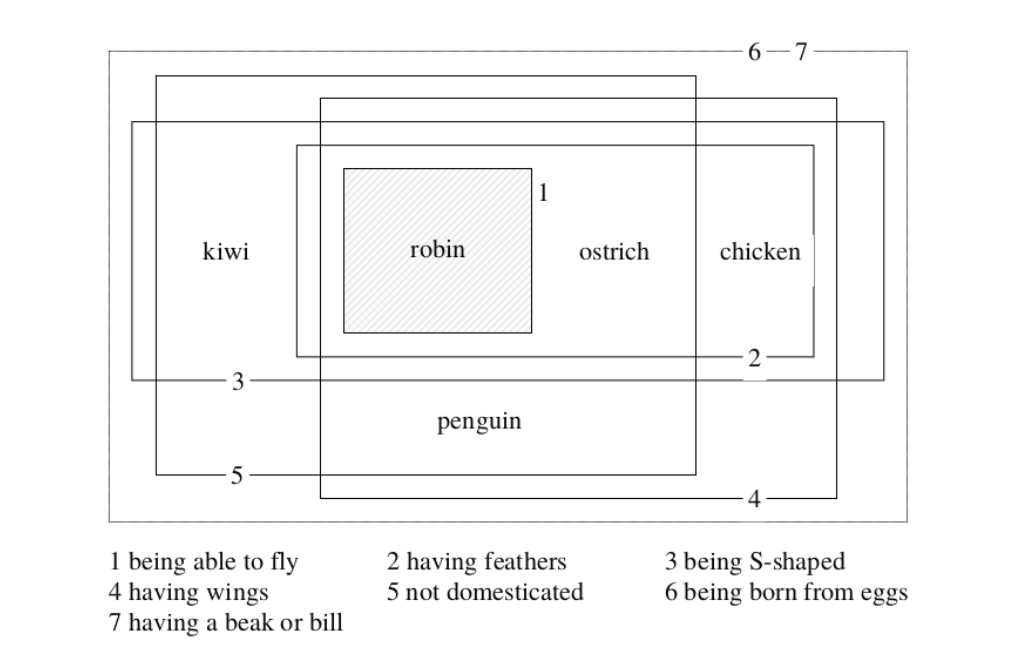
\includegraphics[width=\textwidth]{img/familyres.png}
    \end{figure}
    
    {\scriptsize BECKER, L. \url{https://laurabecker.gitlab.io}}
\end{frame}

\begin{frame}{Example}
  \begin{figure}
    \centering
        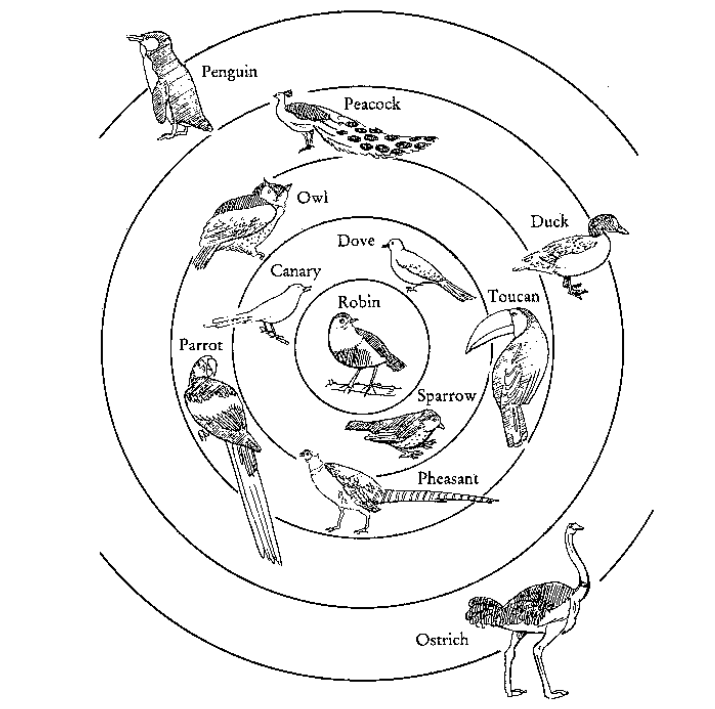
\includegraphics[width=0.65\textwidth]{img/birdstyp.png}
    \end{figure}
    
    {\scriptsize AITCHISON, J. Words in the Mind: An Introduction to the Mental Lexicon. Blackwell: 1987}
\end{frame}

\begin{frame}[fragile]{Defeasibility}

``Reasoning is defeasible when the corresponding argument is \textbf{rationally compelling} but \textbf{not deductively valid}.''\footnote{Koons, R. "Defeasible Reasoning" in The Stanford Encyclopedia of Philosophy.} \pause

\begin{itemize}
  \item Birds fly.\pause
  \begin{itemize}
    \item Counter-examples: penguins, ostriches. \pause
  \end{itemize}
  \item Humans have their hearts on the left side of the chest. \pause
\begin{itemize}
  \item Counter-example: situs inversus.
\end{itemize}
\end{itemize}

\end{frame} 

%

\begin{frame}{Typicality and Defeasible DLs}
\large{Seeing concepts through the lens of prototype theory enables defeasible reasoning. \vspace{2mm}
\begin{itemize}
  \item P1: Birds typically fly.
  \item P2: \textbf{tweety} is a bird.
  \item C: \textbf{tweety} flies.
\end{itemize}
}
\end{frame}

\begin{frame}[fragile]{Typicality and Defeasible DLs}
  \large{Seeing concepts through the lens of prototype theory enables defeasible reasoning. \vspace{2mm}
\begin{itemize}
  \item P1: Birds typically fly.
  \item P2: \textbf{tweety} is a bird.
  \item P3: {\color{red}\textbf{tweety} is a penguin}.
  \item C: \textbf{tweety} {\color{red}does not} fly.
\end{itemize}}
\end{frame}

\begin{frame}[fragile]{Defeasible Knowledge Bases}
  \begin{center}
    \Large{$\Kmc = (\color{gray}{\Amc}, \color{gray}{\Tmc}, {\color{orange}\Dmc}\color{black}{)}$}
  \end{center}

    \vspace{2mm}

    \color{gray}{
    $\dlFont{Bird}({tweety})$
    
    $\dlFont{Bird} \sqsubseteq \dlFont{Animal} \sqcap \exists \dlFont{has}.\dlFont{Wings}$

    $\dlFont{Penguin} \sqsubseteq \dlFont{Bird}$

    $\dlFont{Sparrow} \sqsubseteq \dlFont{Bird}$}

    \Large{
    \color{orange}
    $\dlFont{Bird} \definc \dlFont{Flies}$

    $\dlFont{Bird} \definc \dlFont{Feathered}$

    $\dlFont{Penguin} \definc \lnot \dlFont{Flies}$
  }
\end{frame}

%
% Reasoning task (Defeasible subsumption checking)
%

\begin{frame}[fragile]{Reasoning Task: Defeasible Subsumption Checking}  

\Large{
\begin{itemize}
  \item $\Kmc \models \dlFont{Penguin} \definc \dlFont{Flies}$?
  \item $\Kmc \models \dlFont{Sparrow} \definc \dlFont{Flies}$?
  \item $\Kmc \models \dlFont{Penguin} \definc \dlFont{Feathered}$?
\end{itemize}
}

\end{frame}


%
% Materialisation-based reasoning -- Intro & Notation
%


\begin{frame}[fragile]{Materialisation-based reasoning}
  \begin{center}
    \Large {
      Materialisation
    }

    \LARGE{
  $C \definc D \Rightarrow \lnot C \sqcup D$
    }
\end{center}

\pause
\Large{ $S = \{C_1 \definc D_1, \dots, C_n \definc D_n\}$

$\overline{S} := \sqcap \{\lnot C_i \sqcup D_i \mid C_i \definc D_i \in S\}$
}

\pause 
\begin{center}
  \Large{Materialisation-based Reasoning}
\end{center}

$\Kmc \models_{\mathsf{mat}} C \definc D$ \textbf{iff} $\Kmc \models C \sqcap \overline{S} \sqsubseteq D$ 

$S \subseteq \Dmc$
\end{frame}


\begin{frame}[fragile]{Materialization-based reasoning -- Examples}
\large{
  $\Kmc \models_{\mathsf{mat}} C \definc D$ \textbf{iff} $\Kmc \models C \sqcap \overline{S} \sqsubseteq D$ 

  \vspace{5mm}

  $\Kmc \models \dlFont{Sparrow} \sqcap \materialization{\{\dlFont{Bird} \definc \dlFont{Flies}, \dlFont{Penguin} \definc \lnot \dlFont{Flies}\}} \sqsubseteq \dlFont{Flies}$ 

  \vspace{2mm}

  $\Kmc \models \dlFont{Penguin} \sqcap \overline{\{\dlFont{Penguin} \definc \lnot \dlFont{Flies}\}} \sqsubseteq \lnot \dlFont{Flies}$ 
}
\end{frame}

%
% Rational Reasoning
%

\begin{frame}[fragile]{Rational reasoning}
  \begin{center}
    \large {$C \definc D$ is \textbf{exceptional} \wrt $\Tmc$ and $\Umc \subseteq \Dmc$ iff $\Tmc \models C \sqcap \overline{\Umc} \sqsubseteq \bot$.
    }
\end{center}

\pause
\vspace{0.5cm}
\large{ \color{teal}
  $\Tmc \models \dlFont{Penguin} \sqcap \overline{\Dmc} \sqsubseteq \bot$

  \vspace{0.3cm}
  $\dlFont{Penguin} \definc \dlFont{Flies}$ is exceptional \wrt $\Tmc$ and $\Dmc$
}
\end{frame}

%
% Exceptionality Chain
%
\begin{frame}[fragile]{Exceptionality Chain}

    \large{
    Chain: $\Emc_0 \supset \Emc_1 \supset \dots \supset \Emc_n$
    
  \vspace{0.3cm}

    $\Emc_0 = \Dmc$

    $\Emc_{i + 1} = \{C \definc D \in \Emc_{i} \mid C \definc D \text{ is exceptional \wrt } \Tmc \text{ and } \Emc_i\}$
    }

    \vspace{0.5cm}
    \pause
\begin{center}
  \textbf{Example}
\end{center}

    $\Emc_0 = \{Bird \definc Flies, Bird \definc Feathered, Penguin \definc \lnot Flies\}$
    
    $\Emc_1 = \{Penguin \definc \lnot Flies\}$
    
    $\Emc_2 = \emptyset$
\end{frame}

%
% Rational Reasoning
%

\begin{frame}{Rational Reasoning}
  \large{
  $\Kmc \ratModels C \definc D$ iff $\Tmc \models C \sqcap \overline{\Emc_i} \sqsubseteq D$ 

  For the smallest $i$ \st $C \definc D$ is not exceptional \wrt $\Tmc$ and $\Emc_i$.}
\end{frame}

%
% Rational Reasoning -- Example 1 [1/]
%

\begin{frame}{Examples}
  \begin{tikzpicture}

    % 
    \draw[gray,thick,fill=gray!30,rounded corners] (0, 3) rectangle (4,6); %TBox
        \node[] at (2, 6.4) (TBox) {{\Large $\Tmc$}};

    \draw[gray,thick,fill=gray!30,rounded corners] (5, 3) rectangle (9,6); %DBox E_0
        \node[] at (7, 6.4) (DBox) {{\Large $\Dmc = \Emc_0$}};

    \draw[gray,thick,fill=gray!30,rounded corners] (5.2, 4.5) rectangle (8.8,5.8); %TBox
        \node[] at (9.4, 5.2) (DBox) {{\Large $\Emc_1$}};

    % T - Axioms
    \node [] at (2, 5) (TAxiom) {\begin{tabular}{c} {\large $\dlFont{Penguin} \sqsubseteq \dlFont{Bird}$} \\ ~ \\ {\large $\dlFont{Sparrow} \sqsubseteq \dlFont{Bird}$}  \end{tabular}};

    % E_0 - Axioms
    \node [] at (7, 5.5) (E_0Axiom) {\large $\dlFont{Penguin} \definc \lnot \dlFont{Flies}$};

    % E_1 - Axioms
    \node [] at (7, 3.7) (E_1Axiom) {\begin{tabular}{c} {\large $\dlFont{Bird} \definc \dlFont{Flies}$} \\ ~ \\ {\large $\dlFont{Bird} \definc \dlFont{Feathered}$}  \end{tabular}};        

    \end{tikzpicture}
\end{frame}

%
% Rational Reasoning -- Example 1 [2/]
%

\begin{frame}{Example 1: Sparrows Fly}
  \begin{tikzpicture}

    % 
    \draw[gray,thick,fill=gray!30,rounded corners] (0, 3) rectangle (4,6); %TBox
        \node[] at (2, 6.4) (TBox) {{\Large $\Tmc$}};

    \draw[orange,thick,fill=orange!80,rounded corners] (5, 3) rectangle (9,6); %DBox E_0
        \node[] at (7, 6.4) (DBox) {{\Large $\Dmc = \Emc_0$}};

    \draw[orange!80,thick,fill=orange!80,rounded corners] (5.2, 4.5) rectangle (8.8,5.8); %TBox
        \node[] at (9.4, 5.2) (DBox) {{\Large $\Emc_1$}};

    % T - Axioms
    \node [] at (2, 5) (TAxiom) {\begin{tabular}{c} {\large $\dlFont{Penguin} \sqsubseteq \dlFont{Bird}$} \\ ~ \\ {\large $\dlFont{Sparrow} \sqsubseteq \dlFont{Bird}$}  \end{tabular}};

    % E_0 - Axioms
    \node [] at (7, 5.5) (E_0Axiom) {\large $\dlFont{Penguin} \definc \lnot \dlFont{Flies}$};

    % E_1 - Axioms
    \node [] at (7, 3.7) (E_1Axiom) {\begin{tabular}{c} {\large $\dlFont{Bird} \definc \dlFont{Flies}$} \\ ~ \\ {\large $\dlFont{Bird} \definc \dlFont{Feathered}$}  \end{tabular}};        

    % ENTAILMENT
    \node [] at (5, 1.5) (Entailment) {\large $\Tmc \models \dlFont{Sparrow} \sqcap {\color{orange} \overline{\Emc_0}} \sqsubseteq \dlFont{Flies}$};

    \end{tikzpicture}
\end{frame}



\begin{frame}{Example 2: Inheritance Blocking}
  \begin{tikzpicture}

    % 
    \draw[gray,thick,fill=gray!30,rounded corners] (0, 3) rectangle (4,6); %TBox
        \node[] at (2, 6.4) (TBox) {{\Large $\Tmc$}};

    \draw[gray,thick,fill=gray!30,rounded corners] (5, 3) rectangle (9,6); %DBox E_0
        \node[] at (7, 6.4) (DBox) {{\Large $\Dmc = \Emc_0$}};

    \draw[orange,thick,fill=orange!80,rounded corners] (5.2, 4.5) rectangle (8.8,5.8); %TBox
        \node[] at (9.4, 5.2) (DBox) {{\Large $\Emc_1$}};

    % T - Axioms
    \node [] at (2, 5) (TAxiom) {\begin{tabular}{c} {\large $\dlFont{Penguin} \sqsubseteq \dlFont{Bird}$} \\ ~ \\ {\large $\dlFont{Sparrow} \sqsubseteq \dlFont{Bird}$}  \end{tabular}};

    % E_0 - Axioms
    \node [] at (7, 5.5) (E_0Axiom) {\large $\dlFont{Penguin} \definc \lnot \dlFont{Flies}$};

    % E_1 - Axioms
    \node [] at (7, 3.7) (E_1Axiom) {\begin{tabular}{c} {\large $\dlFont{Bird} \definc \dlFont{Flies}$} \\ ~ \\ {\large $\dlFont{Bird} \definc \dlFont{Feathered}$}  \end{tabular}};        

    % ENTAILMENT
    \node [] at (5, 1.5) (Entailment) {\large $\Tmc \not\models \dlFont{Penguin} \sqcap {\color{orange} \overline{\Emc_1}} \sqsubseteq \dlFont{Feathered}$};

  %\draw [-latex, line width=0.5mm, orange, bend right](5.5,4.5) to (5.5, 1.9);  

    \end{tikzpicture}
\end{frame}

%
% Quantification Neglect [1]
%

\begin{frame}{Example 3: Quantification Neglect}
  \begin{tikzpicture}

    % 
    \draw[gray,thick,fill=gray!30,rounded corners] (0, 3) rectangle (4,6); %TBox
        \node[] at (2, 6.4) (TBox) {{\Large $\Tmc$}};

    \draw[orange,thick,fill=orange!80,rounded corners] (5, 3) rectangle (9,6); %DBox E_0
        \node[] at (7, 6.4) (DBox) {{\Large $\Dmc = \Emc_0$}};

    \draw[orange!80,thick,fill=orange!80,rounded corners] (5.2, 4.5) rectangle (8.8,5.8); %TBox
        \node[] at (9.4, 5.2) (DBox) {{\Large $\Emc_1$}};

    % T - Axioms
    \node [] at (2, 4.5) (TAxiom) {\begin{tabular}{c} {\large $\dlFont{Penguin} \sqsubseteq \dlFont{Bird}$} \\ ~ \\ {\large $\dlFont{Sparrow} \sqsubseteq \dlFont{Bird}$} \\ ~ \\ {\large $\dlFont{Cat} \sqsubseteq \exists \dlFont{eats}.\dlFont{Bird}$} \end{tabular}};

    % E_0 - Axioms
    \node [] at (7, 5.5) (E_0Axiom) {\large $\dlFont{Penguin} \definc \lnot \dlFont{Flies}$};

    % E_1 - Axioms
    \node [] at (7, 3.7) (E_1Axiom) {\begin{tabular}{c} {\large $\dlFont{Bird} \sqsubseteq \dlFont{Flies}$} \\ ~ \\ {\large $\dlFont{Bird} \sqsubseteq \dlFont{Feathered}$}  \end{tabular}};        

    % ENTAILMENT
    \node [] at (5, 1.5) (Entailment) {\large $\Tmc \not\models \dlFont{Cat} \sqcap {\color{orange} \materialization{\Emc_0}} \sqsubseteq \exists \dlFont{eats}.\dlFont{Flies}$};

   % \draw [-latex, line width=0.5mm, bend right, orange](5.5,3) to (4.9,1.9);  

    \end{tikzpicture}
\end{frame}

%%%%%%%%%%%%%%%%%%%%%%%%%%%%%%%%%%%%%%%%%%%%%%%%%
% Section 2: Introduction to Typicality Models  %
%%%%%%%%%%%%%%%%%%%%%%%%%%%%%%%%%%%%%%%%%%%%%%%%%

\section{Typicality Models}

\begin{frame}[fragile]{An overview -- What are typicality models?}

\begin{itemize}
  \item A semantics for reasoning in DDLs based on canonical models. \pause
  \item Originally proposed by $\ELbot$ and recently extended for $\ELIbot$. \pause
  \item The semantics is parametrized with two variables: \textbf{strength} X \textbf{coverage}.
  \begin{itemize}
    \item \textbf{Strength}: related to the materialisation-based reasoning procedure.
    \item \textbf{Coverage}: to which depth the semantics propagate defeasible information (\textbf{propositional} is shallow, while \textbf{nested} is deep).
  \end{itemize}\pause
  \item A typicality upgrade procedure takes the semantics from propositional to nested.
\end{itemize}

\end{frame}

\begin{frame}[fragile]{A Brief Introduction to Canonical Models for the  $\mathcal{EL}$ family}

\large{
  \begin{itemize}
    \item Elements of the domain represent concepts (\ELbot) or sets of concepts (\ELIbot). \pause
    \item We can check subsumption by looking at membership for concept representatives.
    \begin{itemize} \large{
      \item $C \in D^{\CanmodEL}$ iff $\Kmc \models C \sqsubseteq D$
      \item $M \in A^{\CanmodEL}$ iff $\Kmc \models \sqcap_{C \in M}C \sqsubseteq A$}
    \end{itemize}
  \end{itemize}
}

\end{frame}

\begin{frame}[fragile]{Rational Typicality Models for \ELbot}

  \begin{center}
\Large{
  \textbf{Typicality Domains}} 
  
\large{
  $\typel{C}{\Umc}$ represents $C \sqcap \overline{\Umc}$
  
  $\Umc \subseteq \Dmc$
  } 

\pause
\vspace{0.5cm}
\Large{
  \textbf{Defeasible Satisfiability}} 
    
  \large{
    $\Imc \models C \definc D$ iff $\typel{C}{\Emc_i} \in D^{\Imc}$ for every maximal $\Emc_i$ \wrt $C$ in the domain.
    } 
\end{center}
\end{frame}

%
% Rational Domain 
%

\begin{frame}[fragile]{Rational Domain for \ELbot}
  
  \begin{figure}
    \centering
        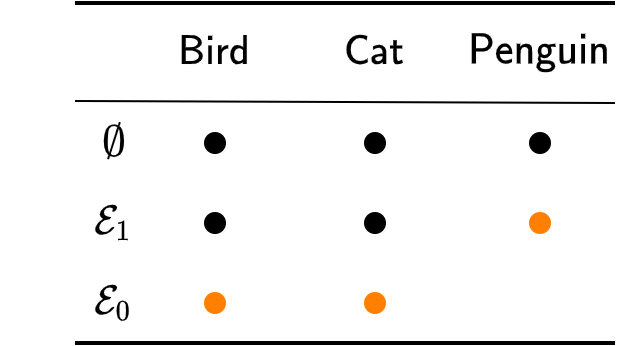
\includegraphics[width=0.7\textwidth]{img/ratmod001.png}
    \end{figure}

\end{frame}

%
% Minimal Rational Domain 
%

\begin{frame}[fragile]{Minimal Typicality Model for \ELbot}

\begin{center}
  { \large 
    $\typel{C}{\Umc} \in D^{\minrattypp}$ iff $\Tmc \models C \sqcap \overline{\Umc} \sqsubseteq D$

    \vspace{0.3cm}
    $(\typel{C}{\Umc},\typel{D}{\emptyset}) \in r^{\minrattypp}$ iff $\Tmc \models C \sqcap \overline{\Umc} \sqsubseteq \exists r.D$.
  }
\end{center}
\pause
\vspace{0.3cm}
\begin{figure}
  \centering
      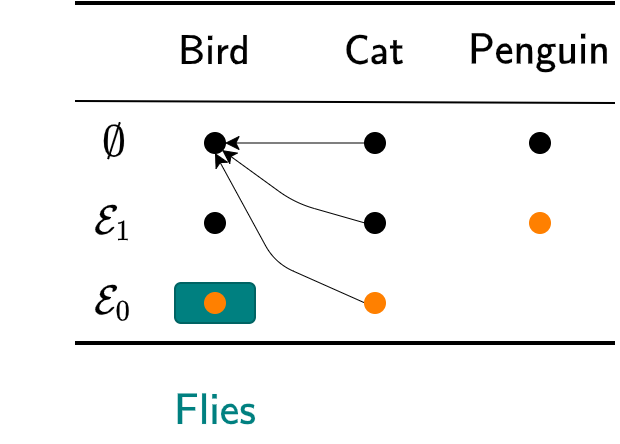
\includegraphics[width=0.7\textwidth]{img/ratmod002.png}
  \end{figure}


\end{frame}

%
% Upgrading Edges
%

\begin{frame}{Upgrading Edges From the Minimal Typicality Model for \ELbot}
  \begin{center}
    { \large 
      $\typel{\dlFont{Cat}}{\Emc_0} \in (\exists \dlFont{eats}.\dlFont{Flies})^{\Imc} \Leftrightarrow \Imc \models \dlFont{Cat} \definc \exists \dlFont{eats}.\dlFont{Flies}$
    }
  \end{center}

  \vspace{0.3cm}
\begin{figure}
  \centering
      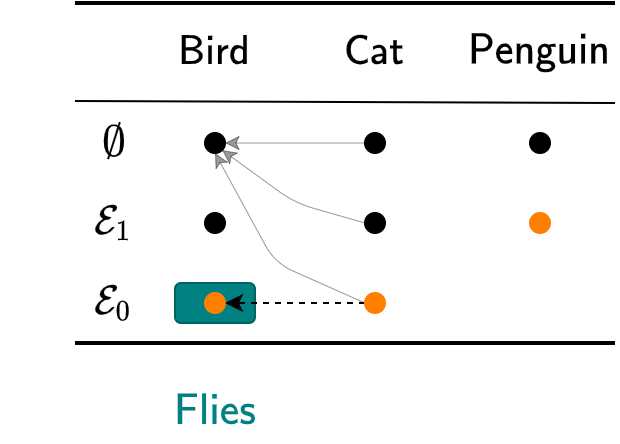
\includegraphics[width=0.7\textwidth]{img/ratmod003.png}
  \end{figure}
\end{frame}

%
% Nested reasoning
%

\begin{frame}{Nested Reasoning}
  
  Upgrade algorithm
  \begin{enumerate}
    \item update an edge,
    \item recover the model property.
  \end{enumerate}

  \vspace{3mm}

  \begin{itemize}
    \item Iterating this procedure until there are no more edges to improve creates a set of \textbf{preferred models} -- \textbf{saturated typicality models}. \pause
    \item This defines \textbf{reasoning of nested coverage}, which \textbf{solves quantification neglect}.
  \end{itemize}

\end{frame}

%%%%%%%%%%%%%%%%%%%%%%%%%%%%%%%%%%%%%%%%%%%
% Section 3: ELI_Bot & Typicality Models  %
%%%%%%%%%%%%%%%%%%%%%%%%%%%%%%%%%%%%%%%%%%%

\section{Introducing Inverse Roles -- $\ELIbot$}


\begin{frame}{$\ELIbot$ -- an overview}
 
  \large{
  \textbf{Inverse roles}: the inverse relation of any given role.
 
  \begin{itemize}
    \item ${r^{-}}^{\Imc} = \{(d,e) \in \Delta^{\Imc} \times \Delta^{\Imc} \mid (e,d) \in r^{\Imc}\}$.
    \item ${\dlFont{parentOf}}^{-} = \dlFont{childrenOf}$.
    \item Expressing value restrictions: $\exists r^{-}.C \sqsubseteq D \equiv C \sqsubseteq \forall r.D$.
    \item Complexity blowup: from linear to \ExpTime.
  \end{itemize}
  }
\end{frame}

%
% Overview
%

\begin{frame}{Three Main Obstacles for $\ELIbot$ TMs}
 
 \Large{
(1.) {\color{orange}Adjusting the domain;}

(2.) Identifying elements in the edges;
 
(3.) Recovering the model property.
}

\end{frame}


%
% Domain
%

\begin{frame}{Adjusting the Domain}
  \begin{center}
    \Large{\ELbot}

      \large{
        $C \sqsubseteq \exists r.D \Rightarrow (C,D) \in r^{\minrattypp}$
    }
  \end{center}
{\large $A \sqsubseteq \exists r.B + A \sqsubseteq \forall r.C$}

  \centering{
  \begin{tikzpicture}
    \draw[orange,thick,fill=orange!30,rounded corners] (1.5, 1.5) rectangle (2.5,2.5); %C Concept
      \node[] at (2,2.8) (CCon) {{\color{orange}$C$}};

    \node[rounded rectangle, fill=white, draw] at (0,1) (A) {$A$};
    \node[rounded rectangle, fill=white, draw] at (2,0) (B) {$B$};
    \node[rounded rectangle, fill=white, draw] at (2,2) (C) {$C$};

    \draw[-latex](A) to (B);
    \draw[-latex](A) to (C);

    \pause

    \draw[orange,thick,fill=orange!30,rounded corners] (5.3, 0.5) rectangle (7.3,2.5);
      \node[] at (6.3,2.8) (CCon) {{\color{orange}$C$}};

    \node[rounded rectangle, fill=white, draw] at (4,1) (A2) {$\{A\}$};
    \node[rounded rectangle, fill=white, draw] at (6,0) (B2) {$\{B\}$};
    \node[rounded rectangle, fill=white, draw] at (6,2) (C2) {$\{C\}$};
    \node[rounded rectangle, fill=white, draw] at (6.5,1) (BC) {$\{B,C\}$};

    \draw[-latex](A2) to (BC);

    \node[] at (3.5, -1) (text) {\large $C \sqsubseteq \exists r.M$ \textbf{ and } $M$ \text{ is maximal } \wrt $\Kmc, C, r \Rightarrow (C,M) \in r^{\minrattypp}$ };
  \end{tikzpicture}}

\end{frame}

%
% Overview 2
%

\begin{frame}{Overview}
  \Large{
 (1.) Adjusting the domain;
 
 (2.) {\color{orange} Identifying elements in the edges;}
  
 (3.) Recovering the model property.
 }
 \end{frame}

%
% Causal Direction of the Edges
%

\begin{frame}{Causal Direction of the Edges}

  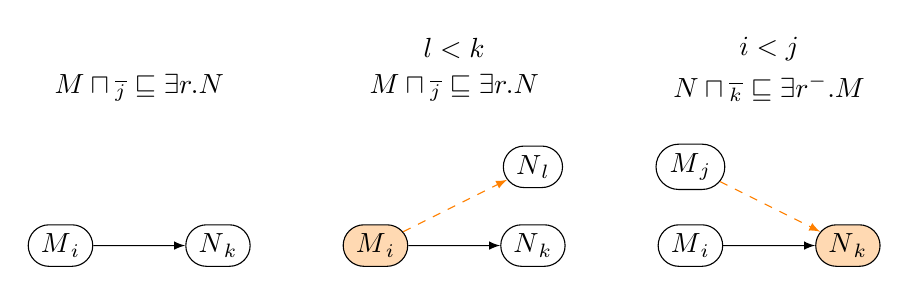
\begin{tikzpicture}

    \node[rounded rectangle, fill=white, draw] at (0,0) (Mi) {$\typel{M}{\Emc_i}$};
    %\node[rounded rectangle, fill=white, draw] at (2,1) (Mj) {$\typel{M}{\Emc_j}$};

    \node[] at (1,2) (N) {$\setconj{M} \sqcap \overline{\Emc_j} \sqsubseteq \exists r.\setconj{N}$};
    \node[rounded rectangle, fill=white, draw] at (2,0) (Nk) {$\typel{N}{\Emc_k}$};
    %\node[rounded rectangle, fill=white, draw] at (2,1) (Nl) {$\typel{N}{\Emc_l}$};
    \draw[-latex](Mi) to (Nk);

    %%% 2 %%%
      \pause

    \node[rounded rectangle, fill=orange!30, draw] at (4,0) (Mi2) {$\typel{M}{\Emc_i}$};

    \node[] at (5,2.5) (lk) {$l < k$};
    \node[] at (5,2) (N2) {$\setconj{M} \sqcap \overline{\Emc_j} \sqsubseteq \exists r.\setconj{N}$};
    \node[rounded rectangle, fill=white, draw] at (6,0) (Nk2) {$\typel{N}{\Emc_k}$};
    \node[rounded rectangle, fill=white, draw] at (6,1) (Nl2) {$\typel{N}{\Emc_l}$};

    \draw[-latex](Mi2) to (Nk2);
    \draw[-latex, dashed, orange](Mi2) to (Nl2);

    %%% 3 %%%
      \pause

    \node[rounded rectangle, fill=white, draw] at (8,0) (Mi3) {$\typel{M}{\Emc_i}$};
    \node[rounded rectangle, fill=white, draw] at (8,1) (Mj) {$\typel{M}{\Emc_j}$};

    \node[] at (9,2.5) (ij) {$i < j$};
    \node[] at (9,2) (ij) {$\setconj{N} \sqcap \overline{\Emc_k} \sqsubseteq \exists r^-.\setconj{M}$};
    \node[rounded rectangle, fill=orange!30, draw] at (10,0) (Nk3) {$\typel{N}{\Emc_k}$};

    \draw[-latex](Mi3) to (Nk3);
    \draw[-latex, dashed, orange](Mj) to (Nk3);

  \end{tikzpicture}

\vspace{5mm}
\begin{center}
  \textbf{Initiator labeling} -- each edge is labeled with $label \subseteq \{s, p\}$.
\end{center}

\end{frame}


% Selecting Candidates + Initiator labeling ?

%
% Overview 3
%

\begin{frame}{Overview}
  \Large{
 (1.) Adjusting the domain;
 
 (2.) Identifying elements in the edges;
  
 (3.) {\color{orange} Recovering the model property}.
 }
 \end{frame}

 %
 % Recovering in ELBot + the problem
 %

 \begin{frame}{Causal Direction of the Edges}

  \begin{tikzpicture}


  \draw[orange,thick,fill=orange!30,rounded corners] (1.5, -0.5) rectangle (2.5,0.5); %C Concept
    \node[] at (2,0.8) (CCon) {{\color{orange}$C$}};

    \node[rounded rectangle, fill=white, draw] at (0,0) (Ai) {$\typel{A}{\Emc_i}$};
    \node[rounded rectangle, fill=white, draw] at (2,0) (Bk) {$\typel{B}{\Emc_k}$};

    \node[] at (1,2) (N) {$\exists r.C \sqsubseteq D$};
    \node[] at (1,1.5) (N) {$\exists r.C \sqsubseteq \exists s.E$};

    \draw[-latex, dashed](Ai) to (Bk);

\pause 

  % Fix #1
  \draw[orange,thick,fill=orange!30,rounded corners] (-0.5, -0.5) rectangle (0.5,0.5); %D Concept
    \node[] at (0,0.8) (DCon) {{\color{orange}$D$}};
  \node[rounded rectangle, fill=white, draw] at (0,0) (Ai) {$\typel{A}{\Emc_i}$};

  \node[rounded rectangle, fill=white, draw] at (2,-1.5) (E) {$\typel{E}{\emptyset}$};
  
  \draw[-latex, dashed](Ai) to (E);

  \node[] at (1,-2.5) (N) {\text{Add \typel{A}{\Emc_i} to $D$}};
  \node[] at (1,-3) (N) {\text{Add edge landing on \typel{E}{\emptyset}}};

  
  %%%%%%%%%%%%%%%% 2 %%%%%%%%%%%%%%%%%
  \pause

  \draw[orange,thick,fill=orange!30,rounded corners] (3.5, -0.5) rectangle (4.5,0.5); %D Concept
    \node[] at (4,0.8) (DCon) {{\color{orange}$D$}};

  \draw[orange,thick,fill=orange!30,rounded corners] (5.5, -0.5) rectangle (6.5,0.5); %C Concept
    \node[] at (6,0.8) (CCon) {{\color{orange}$C$}};

    \node[rounded rectangle, fill=white, draw] at (4,0) (Mi) {$\typel{M}{\Emc_i}$};
    \node[rounded rectangle, fill=white, draw] at (6,0) (Nk) {$\typel{N}{\Emc_k}$};

    \node[] at (5,2) (N) {$\exists r.C \sqsubseteq D$};
    \node[] at (5,1.5) (N) {$D \sqsubseteq \forall r.E$};

    \draw[-latex, dashed](Mi) to (Nk);

\pause 

  % Fix #2
  \node[] at (5,-2.5) (N) {\text{Add $r$ successors to $E$}};

  \draw[teal,thick,fill=teal!30,rounded corners] (5.4, -1) rectangle (6.6,1); %E Concept
    \node[] at (6,0.8) (CCon2) {{\color{orange}$C$}};
    \node[] at (6,-1.3) (CCon2) {{\color{teal}$E$}};

  \draw[orange,thick,fill=orange!30,rounded corners] (5.5, -0.5) rectangle (6.5,0.5); %C Concept

  \node[rounded rectangle, fill=white, draw] at (6,0) (Nk) {$\typel{N}{\Emc_k}$};
  \draw[-latex, dashed](Mi) to (Nk);

  
  
  %%%%%%%%%%%%%%%% 3 %%%%%%%%%%%%%%%%%
  \pause 

  \draw[orange,thick,fill=orange!30,rounded corners] (7.5, -0.5) rectangle (8.5,0.5); %D Concept
    \node[] at (8,0.8) (DCon3) {{\color{orange}$D$}};

  \draw[orange,thick,fill=orange!30,rounded corners] (9.5, -0.5) rectangle (10.5,0.5); %C Concept
    \node[] at (10,0.8) (CCon3) {{\color{orange}$C$}};

    
    \node[rounded rectangle, fill=white, draw] at (8,0) (Mi2) {$\typel{M}{\Emc_i}$};
    \node[rounded rectangle, fill=white, draw] at (10,0) (Nk2) {$\typel{N}{\Emc_k}$};
    \node[rounded rectangle, fill=teal!30, draw] at (9,-1.5) (Nk2) {$\typel{N \cup \{E\}}{\Emc_k}$};

    \draw[-latex, dashed](Mi2) to (Nk2);

  % Fix #3
  \node[] at (8.8,1.5) (N) {\text{Move $r$ edges to include $E$}};

  \end{tikzpicture}

\end{frame}
 

 %
 % Edge Dependency and the solution
 %


%%%%%%%%%%%%%%%%%% NESTED REASONING %%%%%%%%%%%%%%%%%%%%%%%%%%

\section{Nested Reasoning}

%
% Nested reasoning
%

\begin{frame}[fragile] {Nested Reasoning}

\begin{tikzpicture}
  
  \node[] at (1,3) (N) {$\exists r.D \sqcap \exists r.E \sqsubseteq \bot$};

  \draw[orange,thick,fill=orange!30,rounded corners] (1.5, 1) rectangle (2.5,2); %D Concept
    \node[] at (2,2.3) (DCon) {{\color{orange}$D$}};

  \draw[orange,thick,fill=orange!30,rounded corners] (1.5, -2) rectangle (2.5,-1); %E Concept
    \node[] at (2,-2.3) (ECon) {{\color{orange}$E$}};


    \node[rounded rectangle, fill=white, draw] at (0,0) (Ai) {$\typel{A}{\Emc_k}$};

    \node[rounded rectangle, fill=white, draw] at (2,0.5) (B0) {$\typel{B}{\emptyset}$};
    \node[rounded rectangle, fill=white, draw] at (2,1.5) (B1) {$\typel{B}{\Emc_i}$};

    \node[rounded rectangle, fill=white, draw] at (2,-0.5) (C0) {$\typel{C}{\emptyset}$};
    \node[rounded rectangle, fill=white, draw] at (2,-1.5) (C1) {$\typel{C}{\Emc_j}$};

  \draw[-latex] (Ai) to (B0);
  \draw[-latex] (Ai) to (C0);

%%%% Text %%%%

\node[] at (7,3) (text) {\Large \text{Skeptical Reasoning:}};
\node[] at (7,1.5) (text2) {\large $\Kmc \ratModelsnest A \definc B$ \textit{ iff }$\typel{\{A\}}{\Emc_{\min}} \in B^{\Imc}$};
\node[] at (7,1) (text3) {\large \text{In every maximally upgraded $\Imc$}.};

\end{tikzpicture}

\end{frame}

%
% Solving Quantification Neglect
%

\begin{frame}[fragile] {Solving Quantification Neglect}

  \begin{columns}

    \begin{column}{.5\textwidth}
{\Large 
\begin{align*}
  \Tmc = & \{ \dlFont{Penguin} \sqsubseteq \dlFont{Bird}, \\ 
  & \dlFont{Cat} \sqsubseteq \exists \dlFont{eats}.\dlFont{Bird} \} \\ 
  \Dmc = & \{ \dlFont{Penguin} \definc \lnot \dlFont{Flies} \\ 
  & \dlFont{Bird} \definc \dlFont{Flies} \\ 
  & \dlFont{Bird} \definc \dlFont{Feathered} \} 
\end{align*}
}

\end{column}

\begin{column}{.5\textwidth}

  \begin{tikzpicture}
      \draw[teal,thick,fill=teal!30,rounded corners] (1, -1.5) rectangle (3,-0.5); %Flies Concept
      \node[] at (2,-2) (ECon) {{\color{teal}$\dlFont{Flies}$}};

      \node[rounded rectangle, fill=white, draw] at (0,0) (Catd) {$\typel{\{\dlFont{Cat}\}}{\Emc_0}$};
      \node[rounded rectangle, fill=white, draw] at (2,1) (Bird0) {$\typel{\dlFont{Bird}}{\emptyset}$};
      \node[rounded rectangle, fill=white, draw] at (2,-1) (Birdd) {$\typel{\{\dlFont{Bird}\}}{\Dmc}$};

      \draw[-latex] (Catd) to (Bird0);
      \draw[-latex, dashed] (Catd) to (Birdd);

      \node[] at (2,-3) (Catelflies) {{\color{teal}$\{\typel{\dlFont{Cat}}{\Emc_0}\} \in \exists \dlFont{eats}.\dlFont{Flies}^{\Imc}$ }};
      \node[] at (2,-3.5) (CatDCI) {\color{teal}$\Kmc \ratModelsnest \dlFont{Cat} \definc \exists \dlFont{eats}. \dlFont{Flies}$};

  \end{tikzpicture}
\end{column}

\end{columns}
\end{frame}

%
% Conclusions
%

\begin{frame}[fragile] {Summary}

\begin{itemize}
  \item Defeasible reasoning is a robust way to approach typicality within DLs.
  \item Semantics based on typicality models are general enough to model distinct materialisation-based reasoning procedures.
  \item The typicality upgrade procedure defines reasoning of nested coverage, which solves the problem of information spread through roles.
  \item Increase in expressivity come with costs and the procedure depends fundamentally on the simplicity of the canonical structures.
\end{itemize}

\end{frame}

%%%

\begin{frame}[fragile]{Related work not covered here}
\begin{itemize}
  \item Typicality semantics accomodate ABoxes and instance checkings with some adjustments.
  \item There are canonical domains for other materialisation-based reasoning procedures, such as relevant and lexicographic closure.
  \item A full comparison between all the strengths $\times$ coverages for both \ELbot and \ELIbot.
\end{itemize}
\end{frame}

%%%

\begin{frame}[fragile]{Avenues for future research}
  \begin{itemize}
    \item Extending the typicality framework for Horn-DLs.
    \item Including more complex reasoning tasks, such as conjunctive query answering.
    \item Explore the complexity of the calculus for $\ELIbot$.
    \item Implementing typicality-based reasoners.
  \end{itemize}
\end{frame}

\end{document}




